\documentclass[conference,9pt,letterpaper]{IEEEtran}
\usepackage[T1]{fontenc}
\usepackage{newtxtext,newtxmath}
\usepackage{graphicx}
\usepackage{booktabs}
\usepackage{amsmath}
\usepackage{array}
\usepackage{xcolor}
\usepackage{cite}
\usepackage{url}
\usepackage[hidelinks]{hyperref}
\usepackage{stfloats}
\usepackage{balance}
\usepackage{capt-of}
\usepackage{float}
\setcounter{dbltopnumber}{3}
\renewcommand{\dbltopfraction}{0.85}
\renewcommand{\textfraction}{0.10}
\hypersetup{pdftitle={MECC: Single-GPU MoE Inference with Compiler-Guided Three-Tier Expert Caching},pdfauthor={}}
\newcommand{\mecc}{\textsc{MECC}}
\newcommand{\BH}{B_{\mathrm H}}
\newcommand{\BC}{B_{\mathrm C}}
\newcommand{\KH}{K_{\mathrm H}}
\newcommand{\KC}{K_{\mathrm C}}
\newtheorem{proposition}{Proposition}
\title{MECC: Single-GPU MoE Inference with\protect\\Compiler-Guided Three-Tier Expert Caching}
% Anonymous review copy: no author names or affiliation spacer rows.
\author{}
\begin{document}
\maketitle\raggedbottom
\begin{abstract}
Single-GPU mixture-of-experts inference can require weight reads from a cold tier when expert residency is limited. MECC combines a placement interface with joint HBM/host retention and weight delivery. We evaluate its current runtime on one A100 with Mixtral-8x7B and a RAID block device reported as rotational. With uniform initial placement and eight WikiText-2 prompts, MECC takes 7.38~s per decode token, versus 13.04~s for unoptimized streaming and 21.75~s for a fixed-CPU cache. A local recency/frequency adapter takes 7.19~s. A matched independent-cache control takes 32.94~s. These single-run measurements support the retention comparison; profile-guided placement and cross-task adaptation remain separate experiments.
\end{abstract}

\begin{IEEEkeywords}
Mixture of experts, single-GPU inference, expert offloading, three-tier caching, hardware/software co-design.
\end{IEEEkeywords}

\section{Introduction}
Mixture-of-experts (MoE) models activate only a few experts for each token, yet deployment must keep every expert addressable~\cite{shazeer,switch,mixtral,deepseekmoe}. On a single accelerator, the selected expert can be absent from HBM. A server may also assign a task less host memory than the machine physically contains. If the expert set exceeds both allocations, some requests must reach a backing store.

\begin{figure}[!b]
\centering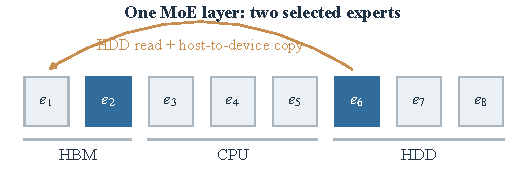
\includegraphics[width=\columnwidth]{measured_figures/intro_compact.pdf}
\caption{Sparse execution still needs the full expert address space. In this layer, the router selects $e_2$ and $e_6$. The HDD-resident $e_6$ must be read through host memory before GPU execution. Shaded experts are selected; tier labels indicate current residency. Schematic.}
\label{fig:intro}
\end{figure}

Figure~\ref{fig:intro} illustrates the resulting weight path. In a local runtime comparison, Streaming takes 13.04~s per output token and fixed-CPU retention takes 21.75~s. Joint retention takes 7.38~s under the same nominal slots. These figures motivate cache coordination; they do not isolate placement or transfer overlap. The readout is slow in absolute terms because HDD-backed demand remains in the critical path.

The operational unit is a selected expert at a particular layer, not a whole model moved for each token. A token passes through successive MoE layers; each layer's gate selects a small set of its own expert IDs. The selected weights must be ready before the expert kernels run. If they are already in HBM, no weight transfer is needed. A host hit needs a host-to-device copy; a cold-tier miss also needs a storage read. The same expert may be selected again by later tokens, making retention useful even when the next layer selects different experts. Figure~\ref{fig:intro} depicts this demand path. It also shows why the host tier matters when it cannot hold the entire expert set assigned to the task.

Multi-GPU expert parallelism can partition experts across resident HBM and move token activations between GPUs~\cite{deepspeedmoe,tutel,flashmoedist}. That is a different capacity point. Single-GPU systems instead choose which weights remain in HBM or host memory and what happens on a miss. Prior work addresses CPU execution, prefetching, cache replacement, and disk delivery~\cite{fiddler,moeinfinity,lightning,ssdllama,flashmoe,offloading}. The design question here is how an independent route profile and the observed route should share those decisions under a task-specific capacity.

This paper makes three contributions. First, it states a compiler interface for ranked per-layer placement under explicit HBM and host allowances. Second, it specifies joint promotion and demotion across the two fast tiers while retaining the original router and FP16 experts. Third, it measures the current single-A100 runtime against matched local controls and separates observed retention gains from placement and adaptation questions that require separate runs.

The system divides decisions by time scale. A route profile gives the compiler a prior over expert demand and determines an initial placement plan. At inference time, the unchanged gate identifies actual demand, and recency updates the identities retained in each tier. The plan fixes capacities within the run; it does not force the runtime to keep an expert that is no longer requested. This separation allows a profile to shorten the initial cold phase while a shared fast-tier cache preserves reuse as inputs change. The evaluation below directly tests the runtime component with uniform initialization. That makes the strongest supported conclusion narrower than the complete design: the measured advantage is from the local joint-retention implementation under the tested slots.

The paper proceeds from the execution and deployment choices in Section~\ref{sec:background} to three capacity and reuse challenges, then presents the system architecture, method, and single-GPU measurements. This order separates the general design from the current implementation evidence.

\clearpage
\section{Background and Related Work}
\label{sec:background}
\subsection{Sparse Execution and Deployment Choices}
For layer $\ell$, a router selects $k_\ell$ of $N_\ell$ experts for each token. Only those experts execute, but any of the $N_\ell$ may be selected by a later token. Switch Transformer and GShard establish the sparse-routing model~\cite{switch,gshard}; Mixtral, DeepSeekMoE, and DeepSeek-V2/V3 show large language-model instances~\cite{mixtral,deepseekmoe,deepseekv2,deepseekv3}. The active parameter count does not by itself specify the required storage capacity.

With enough aggregate GPU memory, expert parallelism places weights on several GPUs and routes token activations to them. DeepSpeed-MoE, Tutel, and MegaBlocks develop execution and scheduling mechanisms for distributed MoE workloads~\cite{deepspeedmoe,tutel,megablocks}. Distributed FlashMoE fuses dispatch, compute, and combine into a persistent kernel~\cite{flashmoedist}; HarMoEny balances token work across GPUs~\cite{harmoeny}. These are relevant deployment alternatives, but their published multi-GPU operator numbers are not single-A100 baselines. Mixtral 8x22B provides a second example of how expert capacity can grow beyond a single card~\cite{mixtral22}.

For one GPU, HBM must also hold dense layers, activations, and KV cache. PagedAttention and SGLang address other parts of the serving-memory and execution problem~\cite{pagedattention,sglang}. CPU memory can retain additional experts; a backing store retains the rest. A miss moves weights from the selected source before the expert kernel executes. FlexGen, DeepSpeed Inference, ZeRO-Infinity, and LLM in a Flash establish related heterogeneous-memory techniques~\cite{flexgen,dsinference,zeroinfinity,llmflash}. PowerInfer exploits activation skew for CPU/GPU inference~\cite{powerinfer}. Their placement and scheduling goals motivate explicit accounting of both resident and temporary copies.

\subsection{Related Expert-Serving Systems}
SwapMoE exposes a tunable memory budget; Fiddler compares CPU expert execution with weight movement; MoE-Lightning pipelines CPU, GPU, and I/O work; and MoE-Infinity uses request-level activation traces~\cite{swapmoe,fiddler,lightning,moeinfinity}. Klotski pipelines expert-aware batches~\cite{klotski}. ExpertFlow predicts routes and schedules tokens, while ProMoE, Pre-gated MoE, and Fate prefetch experts from intermediate signals~\cite{expertflow,promoe,pregated,fate}. DAOP combines data-aware CPU/GPU execution with predictive pre-calculation~\cite{daop}. Those predictors change the information available before a gate. Our demand-only retention rule uses the unchanged gate output.

HOBBIT uses mixed-precision expert loading, and Specter pairs quantization with speculative offloading~\cite{hobbit,specter}. SSD-LLaMA coordinates disk I/O, tiered residency, and execution placement~\cite{ssdllama}. The edge-device FlashMoE learns a recency/frequency replacement rule~\cite{flashmoe}; MoE-CORE combines domain initialization, layer-specific capacities, and prefetch~\cite{core}. ZipMoE adds lossless compression and cache-affinity scheduling~\cite{zipmoe}. These systems overlap individual MECC design axes. Our local RF adapter is not a reproduction of the published FlashMoE system.

MoEpic splits experts into segments and chooses cache allocations; SliceMoE caches precision slices~\cite{moepic,slicemoe}. Mira couples predictive staging with quantized transfers~\cite{mira}. OD-MoE uses on-demand loading across edge nodes; Bevy interleaves concurrent requests during expert fetches~\cite{odmoe,bevy}. HeteGen studies heterogeneous CPU/GPU inference for dense LLMs~\cite{hetegen}. These systems change granularity, prediction, precision, or request scheduling; MECC's measured comparison is limited to the local policies defined in Section~\ref{sec:evaluation}.

The comparison spans three decisions. \emph{Execution location} determines whether to move weights to the GPU or execute an expert on the CPU. Fiddler and DAOP explore this choice~\cite{fiddler,daop}, whereas the measured MECC path executes selected experts on the GPU. \emph{Lookahead} determines when an expert becomes known. ProMoE, Pre-gated MoE, Fate, and Mira expose or predict later demand~\cite{promoe,pregated,fate,mira}; MECC's demand path begins with the original gate output. \emph{Residency} determines which delivered weights survive for reuse. MoE-Infinity, FlashMoE, MoE-CORE, and ZipMoE address this decision with different trace, replacement, initialization, or scheduling mechanisms~\cite{moeinfinity,flashmoe,core,zipmoe}. These axes can coexist in one system, so the experimental controls must identify the particular rule being changed.

The storage regime also affects the comparison. A host-resident expert set mainly exposes PCIe movement or CPU execution. A set larger than the task's fast-tier allowance additionally exposes backing-store reads. SSD-LLaMA and edge FlashMoE explicitly address storage delivery~\cite{ssdllama,flashmoe}. MECC studies HDD-backed demand while combining a placement prior with online HBM/CPU retention.

\section{Motivation and Insights}
\label{sec:challenges}

\subsection{Initial Coverage across Layers}
Figure~\ref{fig:insights}(a) illustrates initial coverage. The expert set is larger than the fast-tier slots assigned to a task. Equal slots per layer can waste capacity when layers receive different fractions of demand. The compiler can rank experts from an independent profile and allocate the next slot where it covers the most expected selections. This is an initial-state decision; it does not change router outputs. Routing locality differs across models and workloads~\cite{routingconsistency}. The current A100 main runs use uniform slots and natural expert order, so their speedup does not measure this insight's profile-guided contribution.

\subsection{Preserving Reuse after Eviction}
Figure~\ref{fig:insights}(b) illustrates reuse across the tier boundary. An HBM victim need not become cold immediately. A later token may select the same expert. Separate HBM and CPU replacement rules can leave a duplicate resident or evict a useful host copy. In a matched local control, independent caches report 47.9\% cold-tier demand and 32.94~s/token; fixed CPU retention reports 31.5\% and 21.75~s/token; joint retention reports 12.5\% and 7.38~s/token. The insight is to treat HBM and host residency as one logical reuse stack: promotion makes room for the HBM victim in host memory. The comparison motivates the runtime rule under the tested quotas; physical bytes and phase-specific I/O remain separate accounting questions.

\subsection{Correcting a Stale Initial State}
Figure~\ref{fig:insights}(c) shows the timing of adaptation. A profile describes a prior workload, not every later request. When the selected expert distribution changes, static residency can keep experts that the new workload rarely uses. The compiler therefore fixes initial capacities and ranked IDs, while online recency changes the resident identities. This division gives the runtime a way to correct a stale prior without modifying the router. A task switch requires two distinct input sets and a measured before/after trace. The present single-A100 main run does not test a switch.

\twocolumn[{
\begin{minipage}{\textwidth}
\centering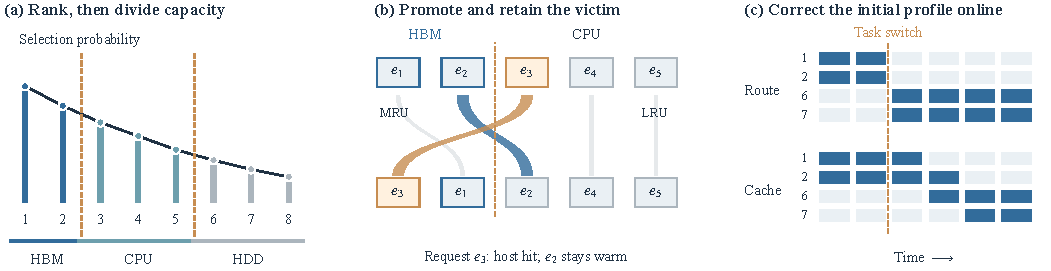
\includegraphics[width=\textwidth]{measured_figures/insights_en.pdf}
\captionof{figure}{Profile-guided placement and online correction. (a) Rank experts within a layer and divide fast-tier capacity at the ranked boundaries. (b) Treat HBM and CPU as one reuse stack: requesting $e_3$ promotes it while retaining the HBM victim $e_2$ in CPU. (c) Update resident identities when the routed expert set changes. All probabilities, states, and time windows are schematic.}
\label{fig:insights}

\section{Overview}
\label{sec:overview}
\centering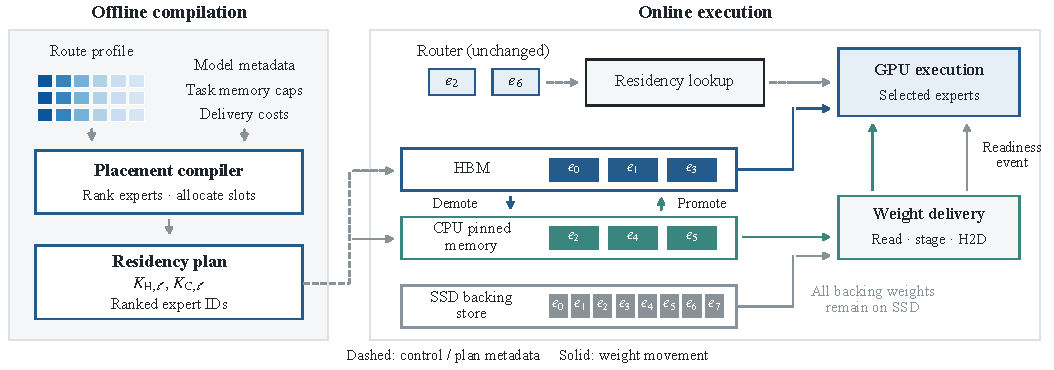
\includegraphics[width=\textwidth]{figures/fig01_overview.pdf}
\captionof{figure}{MECC framework. The placement compiler emits per-layer capacities and ranked IDs. Online execution resolves unchanged router selections against HBM, CPU pinned memory, and HDD, then delivers weights before their GPU consumers. Dashed arrows carry control or plan metadata; solid arrows move weights.}
\label{fig:overview}

\vspace{8pt}
\end{minipage}
}]



Figure~\ref{fig:overview} separates offline compilation from online execution. An independent route profile, model metadata, task memory caps, and delivery costs define the compilation inputs. The output specifies layer capacities and initial expert IDs. Mirrors and staging are charged outside unique primary residency; HDD retains all backing weights.

The unchanged router supplies demand IDs. Residency lookup selects a source tier; the runtime promotes requested experts and demotes HBM victims. The delivery path enforces weight readiness before execution. Layer capacities stay fixed during a run, while expert identities and recency change. Planner controls therefore fix online rules; replacement controls fix quotas and initialization (Section~\ref{sec:mechanisms}).

\section{Method}
\label{sec:method}
\subsection{Compiler: Profile-Guided Placement}
\begin{figure}[H]
\centering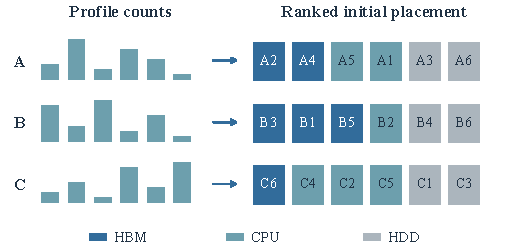
\includegraphics[width=\columnwidth]{measured_figures/method_compile.pdf}
\caption{Compiling layer-specific placement. A, B, and C denote different layers. The compiler keeps each layer's expert identities, ranks its profile counts, and allocates HBM and CPU slots from shared task allowances. Colors identify initial tiers; counts and capacities are schematic.}
\label{fig:compile}
\end{figure}
Figure~\ref{fig:compile} shows the compiler's input and emitted state.
The compiler takes model metadata, memory budgets, delivery costs, and an independent route profile. The profile supplies request probability $p_e$ for each expert. For equal-size experts within a layer, a discrete Zipf model summarizes the ranked probabilities:
\begin{equation}
 q_{\ell,r}=\frac{r^{-\alpha_\ell}}{H_{N_\ell}(\alpha_\ell)},\qquad
 H_n(\alpha)=\sum_{r=1}^{n}r^{-\alpha}.
\end{equation}
Here $q_{\ell,r}$ is conditional on an expert selection in layer $\ell$. Let $w_\ell$ be that layer's fraction of all selections. The global probability is $p_e=w_\ell q_{\ell,r}$, with $\sum_\ell w_\ell=1$. For fixed top-$k$ routing, $w_\ell=k_\ell/\sum_j k_j$. Each rank retains its profiled expert ID. Empirical probabilities can replace the fitted Zipf distribution. Neither representation encodes request order.

Let $x_{e,t}\in\{0,1\}$ indicate the primary tier of expert $e$. The tiers are HBM, CPU, and HDD, denoted by $\mathrm H$, $\mathrm C$, and $\mathrm S$. Residency budgets $\bar B_t$ must exclude buffers and mirrors. The following static objective is a reference model, not a claim that the current planner solves the full problem:
\begin{align}
 \min_x\quad &\sum_e p_e\sum_t x_{e,t}T_t(s_e),\label{eq:placement}\\
 \text{s.t.}\quad&\sum_t x_{e,t}=1,\quad
 \sum_e s_e x_{e,t}\le \bar B_t\quad(t\in\{\mathrm H,\mathrm C\}).\nonumber
\end{align}
The affine model $T_t(s)=a_t+s/b_t$ represents fixed overhead and effective bandwidth. Calibration uses the target machine. Equation~\ref{eq:placement} estimates static delivery cost under the profile. Runtime locality, migration, and overlap are evaluated separately.

\begin{proposition}
Assume equal-size objects, fixed request probabilities, independent tier capacities, and $T_{\mathrm H}\le T_{\mathrm C}\le T_{\mathrm S}$. An optimal static placement fills HBM with the most probable objects, CPU with the next most probable objects, and HDD with the remainder.
\end{proposition}
\noindent\emph{Proof sketch.} Suppose $p_i>p_j$ and object $i$ occupies the slower tier. Exchanging the two objects changes expected cost by $(p_i-p_j)(T_{\mathrm{fast}}-T_{\mathrm{slow}})\le0$. Repeated exchanges produce ranked placement. Filling an empty faster-tier slot also cannot increase cost. The result applies to the stated static model.

The multilayer implementation allocates slots by marginal coverage. Under the Zipf model, a slot covering rank $r$ adds
\begin{equation}
 \Delta_{\ell}(r)=w_\ell q_{\ell,r}.
\end{equation}
This is a coverage score, not the exact latency marginal of Equation~\ref{eq:placement}. Tier-boundary movements can affect both HBM and CPU assignments. The heuristic allocates HBM slots first, then CPU slots from the remaining ranks. At each step it selects the largest next-rank score; ties use layer ID. Expert-ranking ties use expert ID. It stops at the tier's slot cap or exhaustion of experts. Per-layer minima, if enabled, are assigned first and an infeasible minimum allocation must be rejected. A direct scan costs $O(L(S_{\mathrm H}+S_{\mathrm C}))$ after ranking, where $S_t$ is a total slot cap. These rules define the compiler interface. Batched prefill additionally requires distinguishing token selections from distinct expert fetches. The sequential heuristic does not solve the general static objective.

The plan records per-layer capacities, ranked expert IDs, initial tiers, and modeled hit fractions. A missing profile selects natural expert order. The measured runs below use this uniform/natural-order path, so they test the runtime retention and delivery stack rather than the profile compiler. Profile initialization cost and gains require separate matched runs.

\subsection{Runtime: Cross-Tier Retention}
Each layer has ordered HBM and CPU residency maps. An HBM hit updates recency. A CPU hit removes the expert from CPU residency and promotes it to HBM as most recently used. An HDD miss reads the weights into staging before H2D transfer. When HBM is full, its least-recently used expert is demoted to CPU. CPU pressure evicts the least-recently used host resident. The HDD backing weights remain available.

Figure~\ref{fig:retention} starts with HBM $[e_1,e_2]$ and CPU $[e_3,e_4]$, each ordered from MRU to LRU. Requesting $e_3$ promotes it and demotes $e_2$. A later request for $e_2$ hits CPU. This example uses exclusive logical residency. An implementation can keep a CPU mirror to avoid device-to-host (D2H) transfer on eviction. The mirror consumes host memory and is charged separately.

\begin{figure}[H]
\centering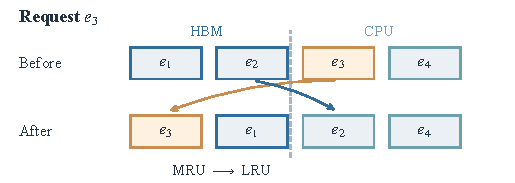
\includegraphics[width=\columnwidth]{measured_figures/method_runtime.pdf}
\caption{One CPU-hit transition. Lists run from MRU to LRU. Requesting $e_3$ promotes it, demotes the HBM victim $e_2$, and preserves both experts in the combined fast-tier set. The dashed line is the capacity boundary.}
\label{fig:retention}
\end{figure}

For a serial demand stream within one layer, concatenate the HBM MRU-to-LRU stack with the CPU MRU-to-LRU stack. Exclusive promotion and victim demotion preserve the corresponding LRU stack of capacity $\KH+\KC$. This reference requires matching initialization, no prefetch or alternative admission, and completed transitions before the next request. It does not imply equivalence to a cache that reallocates capacity across layers, or dominance over static placement.

\subsection{Delivery: Dependency-Aware Overlap}
A correct asynchronous implementation requires a readiness event after each pinned-host copy. The computation stream must wait before consuming the weight. The source buffer must remain live until copy completion, and the resident weight until its last consumer finishes. These are required lifetime rules, including across separate loading and dispatch iterators; the execution stream must enforce them with readiness events.

At batch one, routing reveals the selected IDs only after the current layer's gate. Copying one selected expert may overlap computation of another already-ready expert if kernel and aggregation order permit. This provides no knowledge of a later layer's route. In-flight weights must be protected from eviction. Replacement comparisons must disable predictive prefetch; the overlap control must hold admission, residency, and requests fixed. The available overlap and its exposed critical path remain measurements, rather than an assumed gain from a copy stream.

Figure~\ref{fig:delivery} pairs HBM-resident $e_1$ with HDD-backed $e_3$ from the same gate. HDD read precedes H2D and readiness. Copy completion releases the pinned source; final-consumer completion permits GPU eviction. Useful independent computation determines the available overlap.

\begin{figure}[H]
\centering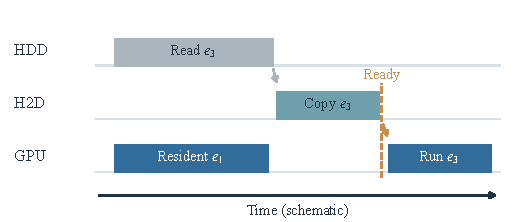
\includegraphics[width=\columnwidth]{measured_figures/method_delivery.pdf}
\caption{Delivery dependencies within one gate's selected set. The GPU can execute resident $e_1$ while $e_3$ is read and copied. A readiness event orders the copied weight before its GPU consumer. Durations are schematic.}
\label{fig:delivery}
\end{figure}

The design requires unchanged weights, selected experts, kernels, and aggregation order. Under these conditions, changing residency preserves the forward computation. The implementation also needs correct synchronization. The validation protocol compares synchronous and asynchronous paths on identical inputs using weight hashes, route selections, logits, tokens, and perplexity; the same protocol isolates transfer scheduling from changes in numerical execution.

\subsection{Implementation and Measurement Contract}
\label{sec:implementation}
Model adapters map layer/expert IDs to immutable FP16 weights. Policies share the loader and router interface. Memory accounting includes physical mirrors and staging buffers.

Physical accounting deduplicates storage identities, not expert IDs: distinct live copies still consume bytes. Let $R_t$ be resident expert bytes, $D_{\mathrm H}$ distinct host mirrors, $S_t$ staging, and $O_t$ other charged allocations. The required constraints are
\begin{align}
 R_{\mathrm C}+D_{\mathrm H}+S_{\mathrm C}+O_{\mathrm C}&\le B_{\mathrm C},\\
 R_{\mathrm H}+W_{\mathrm{dense}}+W_{\mathrm{KV/act}}+S_{\mathrm H}+O_{\mathrm H}&\le B_{\mathrm{GPU}}.
\end{align}
Full mirroring requires $D_{\mathrm H}\ge R_{\mathrm H}$. Residency must be reduced or a mirror-free path validated. Peak measurements must include initialization and transient copies, not only steady residency.

Counters must separate initialization, warmup, prefill, decode, and quality evaluation. TPOT divides decode time by measured intervals; TTFT includes prefill and the first output. Demand-miss share is the fraction of selected-expert arrivals without ready HBM/CPU weights. In-flight prefetch is logged separately. Physical HDD/H2D/D2H bytes use the same phase boundaries. These counters define the same phase boundaries for every policy.

\begin{figure*}[!t]
\centering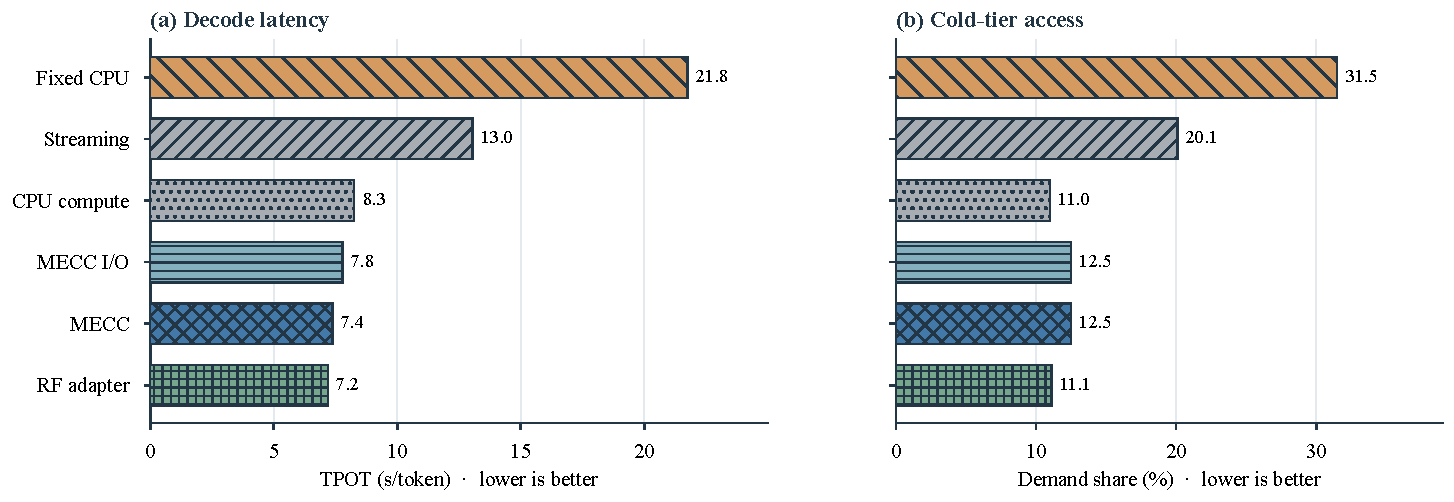
\includegraphics[width=\textwidth]{measured_figures/main.pdf}
\caption{Single-A100 Mixtral-8x7B comparison (eight WikiText-2 prompts, 64 output tokens, one run per policy). (a) Decode time per output token. (b) First-token latency. (c) Reported cold-tier demand share across all instrumented phases, including warmup and perplexity; it is not a decode-only share. All six local policies are shown.}
\label{fig:performance}
\end{figure*}

\section{Evaluation}
\label{sec:evaluation}
\subsection{Testbed and Comparison}
The model is Mixtral-8x7B-Instruct-v0.1 with FP16 expert weights on one A100 80~GB PCIe GPU. The backing store resides on a RAID logical block device reported as rotational (\texttt{ROTA=1}); the physical drives behind the controller have not been inventoried. We call the cold tier HDD as a deployment shorthand. No SSD/NVMe comparison is measured.

The evaluation asks three questions: how much does joint retention change end-to-end latency; where are selected experts found; and how does the host-slot allowance affect both? The counters include warmup and perplexity as well as generation. We therefore report cold-tier demand share as a cache observation, not as a decode-only explanatory variable. TPOT measures the decode interval, whereas TTFT includes the first response.

Each main policy has one completed end-to-end run on the same model revision with nominal expert allowances of 50~GB HBM and 40~GB host memory, four HBM and three host slots per layer, uniform initialization, and cold reads enabled. The input source is WikiText-2 test: eight prompts truncated to 64 input tokens, with 64 generated tokens each. Perplexity uses a 1024-token WikiText-2 sample. Values are single-run point estimates. The nominal host allowance is a planner parameter; mirrors, staging, and page cache are not demonstrated to fit within a physical 40~GB process cap.

The compared policies are unoptimized streaming (\texttt{naive}), fixed-CPU retention (\texttt{swapmoe}), MECC, a local recency/frequency adapter, a CPU-compute adapter, and MECC with an alternative I/O path (\texttt{ours\_io}). The RF and I/O adapters are local implementations, not reproductions of published FlashMoE or SSD-LLaMA. These six runs use one A100 each. There is no measured multi-GPU reference.



\subsection{Single-GPU Latency}
Figure~\ref{fig:performance} reports TPOT of 7.38~s for MECC, 13.04~s for streaming, and 21.75~s for fixed-CPU retention. The corresponding TPOT ratios are 1.77$\times$ and 2.95$\times$. The local RF adapter is slightly faster at 7.19~s; MECC I/O takes 7.78~s and the CPU-compute adapter takes 8.26~s. The cold-tier demand shares are 12.5\% for MECC, 20.1\% for streaming, 31.5\% for fixed CPU, and 11.1\% for RF. These multi-phase counts describe cache behavior, rather than decode-only I/O. The RF adapter has the lowest TTFT and TPOT in this local comparison.

The first-token times are 139.1~s for MECC, 156.9~s for streaming, 174.2~s for fixed CPU, 101.8~s for RF, and 398.4~s for CPU compute. MECC, streaming, fixed CPU, RF, and MECC I/O report perplexity 3.427 on the same 1024-token sample; CPU compute reports 3.432. This quality comparison is specific to that sample. A separate short-window route/logit/token comparison supports the implementation check but is not an independent full-resident reference.

\subsection{Retention Control}
\label{sec:mechanisms}
The independent-cache run matches the main runs' model, nominal slots, input scale, and uniform initialization. Figure~\ref{fig:retention_result} compares independent caching, fixed CPU, and joint MECC retention. Independent caching takes 32.94~s/token and reports 47.9\% cold-tier demand; the fixed-CPU policy takes 21.75~s and reports 31.5\%; MECC takes 7.38~s and reports 12.5\%. The ordering is consistent in both latency and demand sources. Independent caching reaches HBM for 51.9\% of selected experts, fixed CPU reaches HBM for 62.6\%, and MECC reaches HBM for 77.5\%. The CPU shares are 0.3\%, 5.8\%, and 10.0\%, respectively. This comparison supports the joint-retention mechanism under these local policies. Physical host footprints and exposed I/O time still need matched accounting before the entire latency gap can be assigned to replacement alone.

\begin{figure*}[!t]
\begin{minipage}[t]{0.48\textwidth}

\centering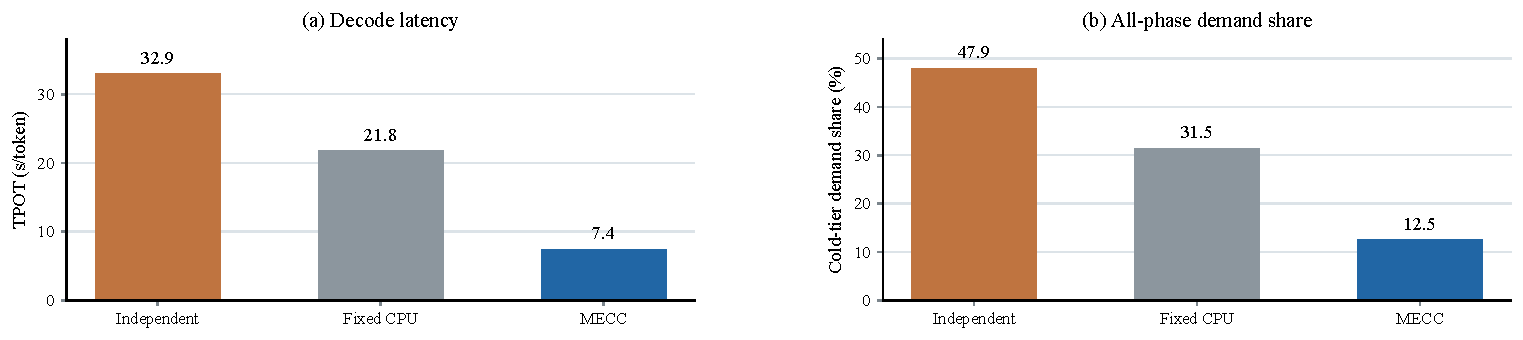
\includegraphics[width=\linewidth]{measured_figures/retention.pdf}
\caption{Matched single-A100 cache-policy control at 50/40~GB nominal allowances, eight WikiText-2 prompts, and 64 output tokens. (a) Decode latency. (b) Selected-expert demand resolved from HBM, CPU, or HDD across all instrumented phases. Independent and fixed-CPU policies are local mechanisms. One run per policy.}
\label{fig:retention_result}

\end{minipage}\hfill
\begin{minipage}[t]{0.48\textwidth}

\centering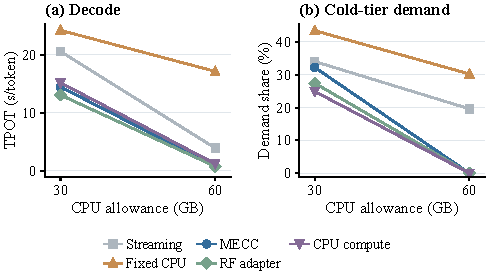
\includegraphics[width=\linewidth]{measured_figures/budget.pdf}
\caption{Nominal CPU-slot sensitivity on one A100. Four WikiText-2 prompts and 16 output tokens per run; 30 and 60~GB are the only two settings shown with the same input source. The earlier 20~GB runs used a different prompt source and are excluded from this comparison. Cold-tier share covers all instrumented phases. One run per point.}
\label{fig:budget}

\end{minipage}
\end{figure*}

\subsection{Host-Slot Sensitivity}
The 30 and 60~GB nominal CPU settings use the same four-prompt, 16-token WikiText-2 protocol within each setting. They are a distinct experiment from the eight-prompt main comparison. At 30~GB, MECC takes 14.46~s/token and reports 32.2\% cold-tier demand; at 60~GB, it takes 0.76~s/token and reports no cold-tier demand. The 60~GB plan has four HBM and four host slots per layer, enough for all eight experts. The RF adapter takes 13.06~s/token at 30~GB and 0.74~s/token at 60~GB, faster than MECC in both settings. Figure~\ref{fig:budget} shows all five local policies at these two settings. The sharp 60~GB drop is a capacity transition: the nominal HBM and host slots together cover all eight experts per layer, so the cold tier is no longer exercised by demand. It should not be interpreted as an HDD optimization gain at that budget.



\balance
\subsection{Reading the Capacity Transition}
The 60~GB plan has four HBM and four CPU slots per layer, covering all eight experts. MECC's zero cold-tier demand is consistent with this slot geometry. It does not mean that the model fits in HBM. At the smaller quota, the cache must decide which experts remain outside the fast tiers, and the replacement rule changes the observed reuse. The main and budget protocols use different prompt/output lengths, so only points within the matched budget protocol belong on the same curve.

\subsection{Scope of the Measurements}
These results are single-run observations on a RAID logical device reporting rotational media. The main comparison uses uniform initialization and does not measure the compiler's profile-guided gain. A true WikiText-2 to GSM8K task-switch sequence has now been implemented, but no completed task-switch result appears in the committed result set. The 20~GB budget runs mix prompt sources and cannot be joined to the 30/60~GB curve. Physical drive identity, physical host-cap equivalence, and multi-GPU resident performance remain separate measurements.

\section{Conclusion}
On one A100 with uniform initial placement, MECC's joint-retention runtime reduces decode latency relative to local streaming, fixed-CPU, and independent-cache controls. The local RF adapter is slightly faster on the main workload. Profile-guided placement, task changes, physical budget equivalence, and multi-GPU tradeoffs require separate evidence before they enter the performance claim.

\clearpage
\nobalance
\IEEEtriggeratref{24}
\bibliographystyle{IEEEtran}
\bibliography{references}
\end{document}
